\documentclass[twoside]{book}

% Packages required by doxygen
\usepackage{fixltx2e}
\usepackage{calc}
\usepackage{doxygen}
\usepackage[export]{adjustbox} % also loads graphicx
\usepackage{graphicx}
\usepackage[utf8]{inputenc}
\usepackage{makeidx}
\usepackage{multicol}
\usepackage{multirow}
\PassOptionsToPackage{warn}{textcomp}
\usepackage{textcomp}
\usepackage[nointegrals]{wasysym}
\usepackage[table]{xcolor}

% Font selection
\usepackage[T1]{fontenc}
\usepackage[scaled=.90]{helvet}
\usepackage{courier}
\usepackage{amssymb}
\usepackage{sectsty}
\renewcommand{\familydefault}{\sfdefault}
\allsectionsfont{%
  \fontseries{bc}\selectfont%
  \color{darkgray}%
}
\renewcommand{\DoxyLabelFont}{%
  \fontseries{bc}\selectfont%
  \color{darkgray}%
}
\newcommand{\+}{\discretionary{\mbox{\scriptsize$\hookleftarrow$}}{}{}}

% Page & text layout
\usepackage{geometry}
\geometry{%
  a4paper,%
  top=2.5cm,%
  bottom=2.5cm,%
  left=2.5cm,%
  right=2.5cm%
}
\tolerance=750
\hfuzz=15pt
\hbadness=750
\setlength{\emergencystretch}{15pt}
\setlength{\parindent}{0cm}
\setlength{\parskip}{3ex plus 2ex minus 2ex}
\makeatletter
\renewcommand{\paragraph}{%
  \@startsection{paragraph}{4}{0ex}{-1.0ex}{1.0ex}{%
    \normalfont\normalsize\bfseries\SS@parafont%
  }%
}
\renewcommand{\subparagraph}{%
  \@startsection{subparagraph}{5}{0ex}{-1.0ex}{1.0ex}{%
    \normalfont\normalsize\bfseries\SS@subparafont%
  }%
}
\makeatother

% Headers & footers
\usepackage{fancyhdr}
\pagestyle{fancyplain}
\fancyhead[LE]{\fancyplain{}{\bfseries\thepage}}
\fancyhead[CE]{\fancyplain{}{}}
\fancyhead[RE]{\fancyplain{}{\bfseries\leftmark}}
\fancyhead[LO]{\fancyplain{}{\bfseries\rightmark}}
\fancyhead[CO]{\fancyplain{}{}}
\fancyhead[RO]{\fancyplain{}{\bfseries\thepage}}
\fancyfoot[LE]{\fancyplain{}{}}
\fancyfoot[CE]{\fancyplain{}{}}
\fancyfoot[RE]{\fancyplain{}{\bfseries\scriptsize Generated by Doxygen }}
\fancyfoot[LO]{\fancyplain{}{\bfseries\scriptsize Generated by Doxygen }}
\fancyfoot[CO]{\fancyplain{}{}}
\fancyfoot[RO]{\fancyplain{}{}}
\renewcommand{\footrulewidth}{0.4pt}
\renewcommand{\chaptermark}[1]{%
  \markboth{#1}{}%
}
\renewcommand{\sectionmark}[1]{%
  \markright{\thesection\ #1}%
}

% Indices & bibliography
\usepackage{natbib}
\usepackage[titles]{tocloft}
\setcounter{tocdepth}{3}
\setcounter{secnumdepth}{5}
\makeindex

% Hyperlinks (required, but should be loaded last)
\usepackage{ifpdf}
\ifpdf
  \usepackage[pdftex,pagebackref=true]{hyperref}
\else
  \usepackage[ps2pdf,pagebackref=true]{hyperref}
\fi
\hypersetup{%
  colorlinks=true,%
  linkcolor=blue,%
  citecolor=blue,%
  unicode%
}

% Custom commands
\newcommand{\clearemptydoublepage}{%
  \newpage{\pagestyle{empty}\cleardoublepage}%
}

\usepackage{caption}
\captionsetup{labelsep=space,justification=centering,font={bf},singlelinecheck=off,skip=4pt,position=top}

%===== C O N T E N T S =====

\begin{document}

% Titlepage & ToC
\hypersetup{pageanchor=false,
             bookmarksnumbered=true,
             pdfencoding=unicode
            }
\pagenumbering{roman}
\begin{titlepage}
\vspace*{7cm}
\begin{center}%
{\Large Genetics \\[1ex]\large 1 }\\
\vspace*{1cm}
{\large Generated by Doxygen 1.8.11}\\
\end{center}
\end{titlepage}
\clearemptydoublepage
\tableofcontents
\clearemptydoublepage
\pagenumbering{arabic}
\hypersetup{pageanchor=true}

%--- Begin generated contents ---
\chapter{Hierarchical Index}
\section{Class Hierarchy}
This inheritance list is sorted roughly, but not completely, alphabetically\+:\begin{DoxyCompactList}
\item \contentsline{section}{Allele}{\pageref{class_allele}}{}
\item \contentsline{section}{Coleman\+X\+M\+L\+Parser}{\pageref{class_coleman_x_m_l_parser}}{}
\item \contentsline{section}{Gene}{\pageref{class_gene}}{}
\item \contentsline{section}{Genetics\+Sim\+Data\+Parser}{\pageref{class_genetics_sim_data_parser}}{}
\item \contentsline{section}{I\+File\+Parser}{\pageref{struct_i_file_parser}}{}
\item \contentsline{section}{I\+Observable}{\pageref{class_i_observable}}{}
\begin{DoxyCompactList}
\item \contentsline{section}{Love\+Chamber}{\pageref{class_love_chamber}}{}
\end{DoxyCompactList}
\item \contentsline{section}{I\+Observer$<$ T $>$}{\pageref{struct_i_observer}}{}
\begin{DoxyCompactList}
\item \contentsline{section}{Stat\+Counter}{\pageref{class_stat_counter}}{}
\end{DoxyCompactList}
\item \contentsline{section}{I\+Observer$<$ Organism $>$}{\pageref{struct_i_observer}}{}
\begin{DoxyCompactList}
\item \contentsline{section}{Stat\+Counter}{\pageref{class_stat_counter}}{}
\end{DoxyCompactList}
\item \contentsline{section}{Observable$<$ T $>$}{\pageref{class_observable}}{}
\item \contentsline{section}{Observable$<$ Organism $>$}{\pageref{class_observable}}{}
\begin{DoxyCompactList}
\item \contentsline{section}{Love\+Chamber}{\pageref{class_love_chamber}}{}
\end{DoxyCompactList}
\item \contentsline{section}{Organism}{\pageref{class_organism}}{}
\item \contentsline{section}{Simulation}{\pageref{class_simulation}}{}
\end{DoxyCompactList}

\chapter{Class Index}
\section{Class List}
Here are the classes, structs, unions and interfaces with brief descriptions\+:\begin{DoxyCompactList}
\item\contentsline{section}{\hyperlink{class_allele}{Allele} \\*Models the alleles of a \hyperlink{class_gene}{Gene} }{\pageref{class_allele}}{}
\item\contentsline{section}{\hyperlink{class_coleman_x_m_l_parser}{Coleman\+X\+M\+L\+Parser} \\*Wraps behavior of \hyperlink{class_genetics_sim_data_parser}{Genetics\+Sim\+Data\+Parser} }{\pageref{class_coleman_x_m_l_parser}}{}
\item\contentsline{section}{\hyperlink{class_empty_container_exception}{Empty\+Container\+Exception} \\*Exception for empty containers }{\pageref{class_empty_container_exception}}{}
\item\contentsline{section}{\hyperlink{class_gene}{Gene} \\*Handles pairs of \hyperlink{class_allele}{Allele} }{\pageref{class_gene}}{}
\item\contentsline{section}{\hyperlink{class_genetics_sim_data_parser}{Genetics\+Sim\+Data\+Parser} }{\pageref{class_genetics_sim_data_parser}}{}
\item\contentsline{section}{\hyperlink{struct_i_observer}{I\+Observer$<$ T $>$} \\*The \hyperlink{struct_i_observer}{I\+Observer} class is an interface for observers }{\pageref{struct_i_observer}}{}
\item\contentsline{section}{\hyperlink{class_love_chamber}{Love\+Chamber} \\*Handles mating between Organisms }{\pageref{class_love_chamber}}{}
\item\contentsline{section}{\hyperlink{class_malformed_file_exception}{Malformed\+File\+Exception} \\*Exception for malformed files }{\pageref{class_malformed_file_exception}}{}
\item\contentsline{section}{\hyperlink{class_observable}{Observable$<$ T $>$} \\*The \hyperlink{class_observable}{Observable} class is an interface for observable objects }{\pageref{class_observable}}{}
\item\contentsline{section}{\hyperlink{class_organism}{Organism} \\*Living thing }{\pageref{class_organism}}{}
\item\contentsline{section}{\hyperlink{class_simulation}{Simulation} \\*Handles the main thread of execution for the genetic simulation }{\pageref{class_simulation}}{}
\item\contentsline{section}{\hyperlink{class_stat_counter}{Stat\+Counter} \\*Records statistical data of Organisms }{\pageref{class_stat_counter}}{}
\end{DoxyCompactList}

\chapter{Class Documentation}
\hypertarget{class_coleman_x_m_l_parser}{}\section{Coleman\+X\+M\+L\+Parser Class Reference}
\label{class_coleman_x_m_l_parser}\index{Coleman\+X\+M\+L\+Parser@{Coleman\+X\+M\+L\+Parser}}


The \hyperlink{class_coleman_x_m_l_parser}{Coleman\+X\+M\+L\+Parser} class wraps behavior of \hyperlink{class_genetics_sim_data_parser}{Genetics\+Sim\+Data\+Parser}.  




{\ttfamily \#include $<$Coleman\+X\+M\+L\+Parser.\+h$>$}

\subsection*{Public Member Functions}
\begin{DoxyCompactItemize}
\item 
\hypertarget{class_coleman_x_m_l_parser_a8eda751b3cb0b3f94add5a24fddacbc1}{}{\bfseries Coleman\+X\+M\+L\+Parser} (const string \&filename)\label{class_coleman_x_m_l_parser_a8eda751b3cb0b3f94add5a24fddacbc1}

\item 
void \hyperlink{class_coleman_x_m_l_parser_ae168a5ae05ee145556a7b1f612fde3ea}{parse\+File} (std\+::vector$<$ \hyperlink{class_organism}{Organism} $>$ \&organisms)
\begin{DoxyCompactList}\small\item\em Reads organism data from a file into a vector of organisms. \end{DoxyCompactList}\end{DoxyCompactItemize}


\subsection{Detailed Description}
The \hyperlink{class_coleman_x_m_l_parser}{Coleman\+X\+M\+L\+Parser} class wraps behavior of \hyperlink{class_genetics_sim_data_parser}{Genetics\+Sim\+Data\+Parser}. 

This class acts as a wrapper around Dr. Coleman\textquotesingle{}s \hyperlink{class_genetics_sim_data_parser}{Genetics\+Sim\+Data\+Parser} class. It takes a filename which should contain organism data and then stores that data in a supplied container. \begin{DoxySeeAlso}{See also}
\hyperlink{class_genetics_sim_data_parser}{Genetics\+Sim\+Data\+Parser} 
\end{DoxySeeAlso}


\subsection{Member Function Documentation}
\hypertarget{class_coleman_x_m_l_parser_ae168a5ae05ee145556a7b1f612fde3ea}{}\index{Coleman\+X\+M\+L\+Parser@{Coleman\+X\+M\+L\+Parser}!parse\+File@{parse\+File}}
\index{parse\+File@{parse\+File}!Coleman\+X\+M\+L\+Parser@{Coleman\+X\+M\+L\+Parser}}
\subsubsection[{parse\+File}]{\setlength{\rightskip}{0pt plus 5cm}void Coleman\+X\+M\+L\+Parser\+::parse\+File (
\begin{DoxyParamCaption}
\item[{std\+::vector$<$ {\bf Organism} $>$ \&}]{organisms}
\end{DoxyParamCaption}
)}\label{class_coleman_x_m_l_parser_ae168a5ae05ee145556a7b1f612fde3ea}


Reads organism data from a file into a vector of organisms. 


\begin{DoxyParams}{Parameters}
{\em organisms} & The vector to store the organisms in \\
\hline
{\em expected\+Count} & The expected organism count in the data file \\
\hline
\end{DoxyParams}
\begin{DoxySeeAlso}{See also}
\hyperlink{class_organism}{Organism} 
\end{DoxySeeAlso}


The documentation for this class was generated from the following files\+:\begin{DoxyCompactItemize}
\item 
Genetics/Coleman\+X\+M\+L\+Parser.\+h\item 
Genetics/Coleman\+X\+M\+L\+Parser.\+cpp\end{DoxyCompactItemize}

\hypertarget{struct_i_file_parser}{}\section{I\+File\+Parser Struct Reference}
\label{struct_i_file_parser}\index{I\+File\+Parser@{I\+File\+Parser}}


The \hyperlink{struct_i_file_parser}{I\+File\+Parser} struct provides an interface for reading genotype information from various file formats.  




{\ttfamily \#include $<$File\+Parser.\+h$>$}

Inheritance diagram for I\+File\+Parser\+:\begin{figure}[H]
\begin{center}
\leavevmode
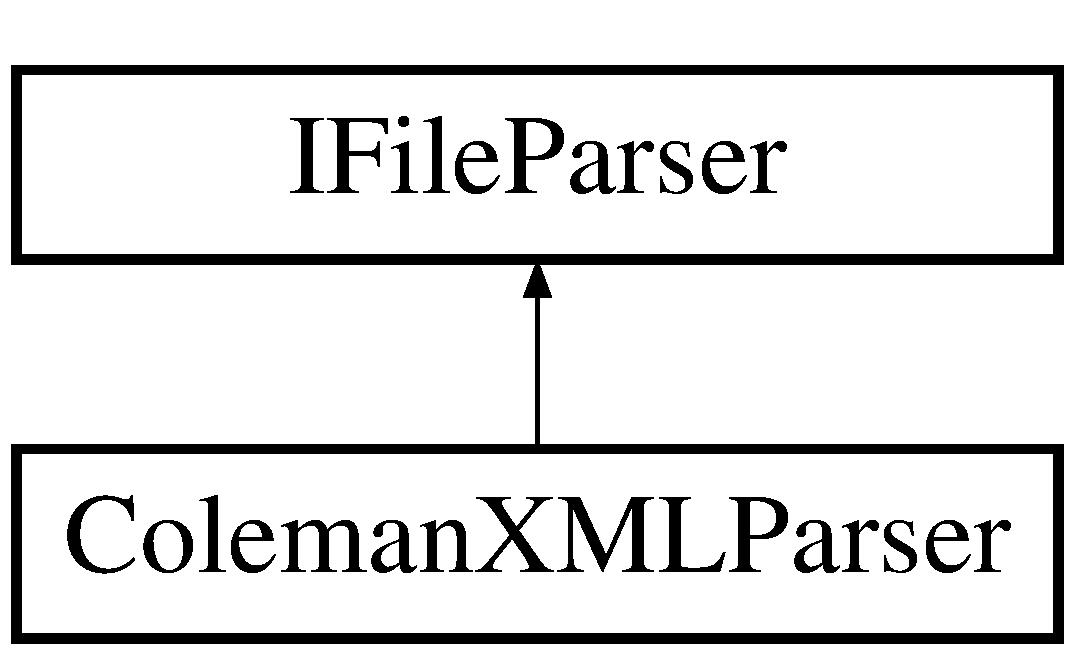
\includegraphics[height=2.000000cm]{struct_i_file_parser}
\end{center}
\end{figure}
\subsection*{Public Member Functions}
\begin{DoxyCompactItemize}
\item 
virtual void {\bfseries parse\+File} (std\+::vector$<$ std\+::string $>$ \&genotypes, int expected\+Count)=0\hypertarget{struct_i_file_parser_a3507bb9e7f103b5bbcc64f1077087fc3}{}\label{struct_i_file_parser_a3507bb9e7f103b5bbcc64f1077087fc3}

\end{DoxyCompactItemize}


\subsection{Detailed Description}
The \hyperlink{struct_i_file_parser}{I\+File\+Parser} struct provides an interface for reading genotype information from various file formats. 

The documentation for this struct was generated from the following file\+:\begin{DoxyCompactItemize}
\item 
Genetics/File\+Parser.\+h\end{DoxyCompactItemize}

%--- End generated contents ---

% Index
\backmatter
\newpage
\phantomsection
\clearemptydoublepage
\addcontentsline{toc}{chapter}{Index}
\printindex

\end{document}
